\chapter{Porównanie}

\begin{figure}[h!]
\centering
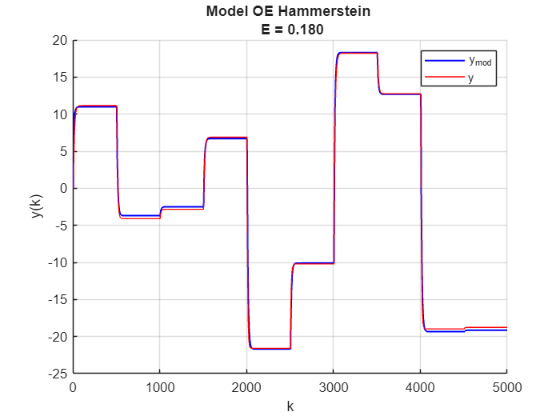
\includegraphics[width=0.7\textwidth]{pictures/model_hammersteina}
\caption{Model Hammersteina - następniki nieliniowe..}
\end{figure}

\begin{figure}[h!]
\centering
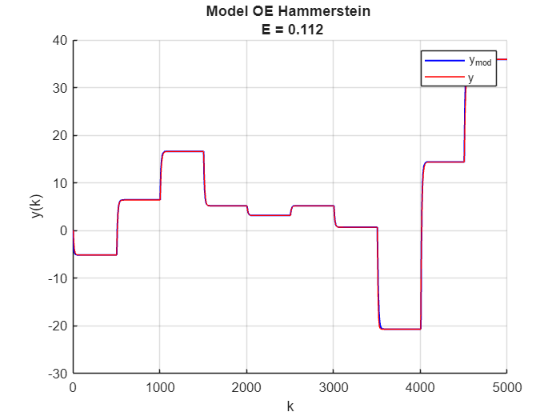
\includegraphics[width=0.7\textwidth]{pictures/model_hammersteina_lin}
\caption{Model Hammersteina - następniki liniowe.}
\end{figure}

\newpage

\begin{figure}[h!]
\centering
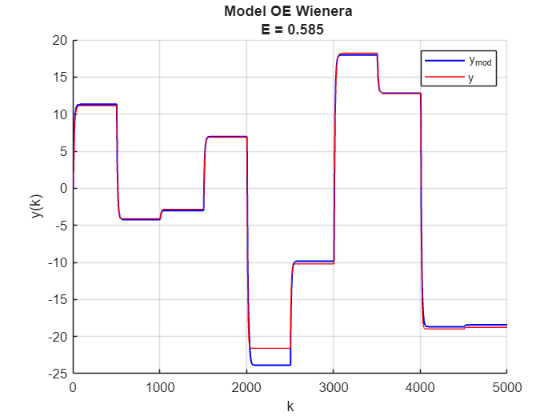
\includegraphics[width=0.7\textwidth]{pictures/model_wienera}
\caption{Model Wienera - następniki nieliniowe.}
\end{figure}

\begin{figure}[h!]
\centering
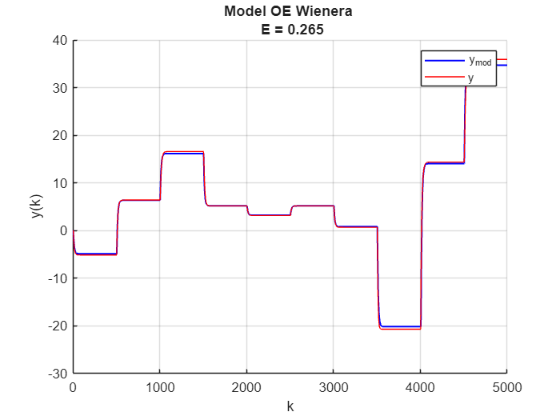
\includegraphics[width=0.7\textwidth]{pictures/model_wienera_lin}
\caption{Model Wienera - następniki liniowe.}
\end{figure}

\newpage

\begin{figure}[h!]
\centering
\includegraphics[width=\textwidth]{pictures/model_OE}
\caption{Model liniowy.}
\end{figure}

Zastosowania modeli zarówno Hammersteina, jak i Wienera przynosi duże korzyści w stosunku do samego modelu liniowego. Natomiast zastosowanie nieliniowych funkcji w następnikach reguł modelu Takagi-Sugeno pozwala zredukować liczbę zbiorów rozmytych nieznacznie tracąc na dokładności.